\documentclass[11pt,a4paper]{article}
\usepackage[margin=2.4cm]{geometry}
\usepackage[T1]{fontenc}
\usepackage[utf8]{inputenc}
\usepackage{amsmath,amssymb,amsthm,mathtools,bm}
\usepackage{booktabs,array,enumitem}
\usepackage{xcolor}
\usepackage{tikz}
\usetikzlibrary{arrows.meta,calc,positioning,decorations.pathreplacing,patterns,shapes.geometric,fit}
\usepackage{pgfplots}
\pgfplotsset{compat=1.17}
\usepackage[most]{tcolorbox}
\tcbuselibrary{theorems,breakable,skins}
\usepackage{algpseudocode}
\usepackage{listings}
\usepackage[colorlinks=true,linkcolor=blue!50!black,urlcolor=blue!50!black]{hyperref}

\definecolor{orng}{RGB}{245,150,40}
\definecolor{cloud}{RGB}{190,215,240}

% ---------- macros ----------
\newcommand{\slides}[1]{\texorpdfstring{\hfill{\normalfont\small\emph{(slides #1)}}}{ (slides #1)}}
\newcommand{\x}{\bm{x}}
\newcommand{\y}{\bm{y}}
\newcommand{\z}{\bm{z}}
\newcommand{\w}{\bm{\omega}}
\newcommand{\dd}{\,\mathrm{d}}
\newcommand{\R}{\mathbb{R}}
\newcommand{\Sph}{\mathbb{S}^2}
\newcommand{\Tr}{T}
\theoremstyle{remark}\newtheorem*{remark}{Remark}

% ---------- boxes ----------
\newtcbtheorem[number within=section]{definition}{Definition}
 {enhanced,breakable,colback=gray!5,colframe=black!70,fonttitle=\bfseries,coltitle=white,
  attach boxed title to top left={yshift=-2mm},boxed title style={colback=black!70},
  before skip=10pt,after skip=10pt}{def}
\newtcbtheorem[use counter from=definition]{lemma}{Lemma}
 {enhanced,breakable,colback=green!4,colframe=green!45!black,fonttitle=\bfseries,coltitle=white,
  attach boxed title to top left={yshift=-2mm},boxed title style={colback=green!45!black},
  before skip=10pt,after skip=10pt}{lem}
\newtcbtheorem[use counter from=definition]{theorem}{Theorem}
 {enhanced,breakable,colback=red!4,colframe=red!55!black,fonttitle=\bfseries,coltitle=white,
  attach boxed title to top left={yshift=-2mm},boxed title style={colback=red!55!black},
  before skip=10pt,after skip=10pt}{thm}
\newtcbtheorem[use counter from=definition]{proposition}{Proposition}
 {enhanced,breakable,colback=orange!5,colframe=orange!70!black,fonttitle=\bfseries,coltitle=white,
  attach boxed title to top left={yshift=-2mm},boxed title style={colback=orange!70!black},
  before skip=10pt,after skip=10pt}{prop}
\newtcbtheorem[use counter from=definition]{corollary}{Corollary}
 {enhanced,breakable,colback=purple!4,colframe=purple!60!black,fonttitle=\bfseries,coltitle=white,
  attach boxed title to top left={yshift=-2mm},boxed title style={colback=purple!60!black},
  before skip=10pt,after skip=10pt}{cor}
\newtcbtheorem[use counter from=definition]{example}{Example}
 {enhanced,breakable,colback=yellow!7,colframe=yellow!50!black,fonttitle=\bfseries,coltitle=white,
  attach boxed title to top left={yshift=-2mm},boxed title style={colback=yellow!50!black},
  before skip=10pt,after skip=10pt}{ex}
\newtcbtheorem[use counter from=definition]{algorithm}{Algorithm}
 {enhanced,breakable,colback=teal!4,colframe=teal!55!black,fonttitle=\bfseries,coltitle=white,
  attach boxed title to top left={yshift=-2mm},boxed title style={colback=teal!55!black},
  before skip=10pt,after skip=10pt}{alg}
\newtcolorbox{intuition}{enhanced,breakable,colback=blue!6,colframe=blue!65!black,
  fonttitle=\bfseries,title=Intuition,coltitle=white,before skip=8pt,after skip=12pt}

% placeholder for photos that are hard to reproduce
\newcommand{\photo}[3]{%  slide, caption, height(cm)
 \begin{center}
 \begin{tikzpicture}
  \draw[dashed,gray,thick] (0,0) rectangle (0.88\linewidth,#3 cm);
  \node[gray,align=center] at (0.44\linewidth,#3/2) {\textbf{[ Insert image from slide #1 ]}};
 \end{tikzpicture}\\[2pt]
 {\small\emph{#2}}
 \end{center}}

\pgfplotsset{every axis/.append style={font=\small,width=0.82\linewidth,height=5.6cm,grid=major,
  grid style={gray!25}}}

% cylinder slab pic
\tikzset{pics/slab/.style={code={
  \draw[fill=white] (0,0) ellipse (0.22 and 0.6);
  \fill[white] (0,0.6) rectangle (1.4,-0.6);
  \draw (0,0.6)--(1.4,0.6); \draw (0,-0.6)--(1.4,-0.6);
  \draw[fill=gray!8] (1.4,0) ellipse (0.22 and 0.6);
  \foreach \px/\py/\pr in {0.3/0.25/0.07,0.55/-0.3/0.05,0.8/0.2/0.06,1.0/-0.1/0.07,1.2/0.3/0.04,0.45/0.0/0.05,0.95/-0.4/0.05,1.25/-0.25/0.06}
     \draw[fill=white,gray] (\px,\py) circle (\pr);
}}}

\title{\textbf{Foundations of Spatial AI}\\[4pt] Lecture 07 --- Volume Rendering\\[4pt]
\large Detailed lecture notes}
\author{Notes based on the slides of E.~Giacomini and L.~Di Giammarino\\ Sapienza University of Rome, October 13, 2026}
\date{}

\begin{document}
\maketitle
\begin{center}
\begin{minipage}{0.9\linewidth}
\small\textbf{About these notes.} The structure follows the slide deck; every section title is (nearly) the slide title, with the slide range in italics. No companion book chapter was provided, so the formal material (definitions, propositions, proofs) is derived from the equations on the slides, and I flag explicitly whenever I add something that is not on the slides (for instance the normalisation of the phase function, or the partition-of-unity identity for the ray-marching weights). Two typos on the slides are corrected in remarks (slides 53 and 68). Photographs are left as blank frames with the slide number and the caption to use. All figures are original TikZ/pgfplots.
\end{minipage}
\end{center}
\tableofcontents
\newpage

%=====================================================================
\section{From One View to Many\slides{2--3}}
%=====================================================================
\subsection{From One View to Many\slides{2}}

\photo{2}{Input images, 3D surface, light \& reflectance and cameras recovered by IDR. Figure credits: Yariv et al.}{5.5}

The lectures so far dealt with one or two views (single-view depth, stereo). From now on we have \emph{many} images of the same scene with known (or estimated) cameras, and the goal is stated on the slide:

\begin{definition}{Multi-view objective}{objective}
Find a \emph{learnable} 3D representation $\mathcal{S}_\theta$ that is \emph{consistent with all observed views}: if we render $\mathcal{S}_\theta$ from the camera of image $I_k$, we should reproduce $I_k$, for every $k$.
\end{definition}

\begin{intuition}
Think of the scene as an unknown object hidden in a box and the photos as ``shadows'' of it. Any representation (mesh, points, field, \dots) is acceptable as long as, when we ``shine light'' through it from camera $k$, we get image $k$ back. The words \emph{learnable} and \emph{rendering} are the two ingredients of the course from here on: the representation has parameters we can optimise, and a differentiable renderer links it to pixels. The next lectures cover different representations and optimisation methods; \textbf{today we study the renderer} for one family of representations (density fields).
\end{intuition}

\begin{figure}[h]
\centering
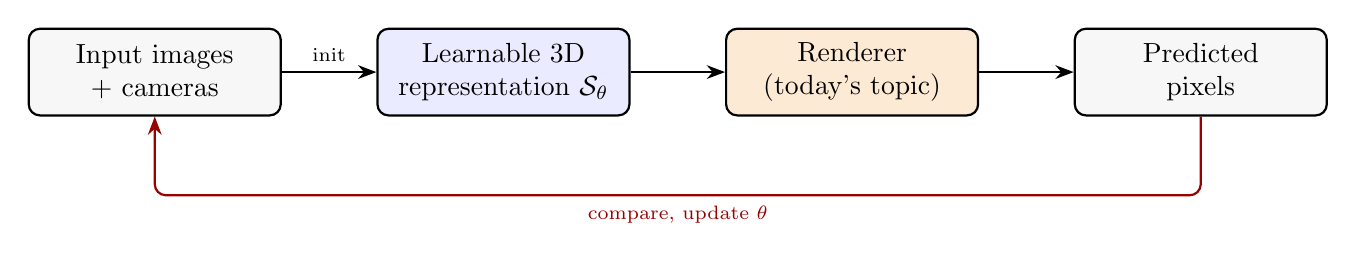
\begin{tikzpicture}[node distance=1.2cm,>=Stealth,
  box/.style={draw,rounded corners,thick,minimum width=3.2cm,minimum height=1.1cm,align=center,fill=gray!6}]
 \node[box] (img) {Input images\\+ cameras};
 \node[box,right=of img,fill=blue!8] (rep) {Learnable 3D\\representation $\mathcal{S}_\theta$};
 \node[box,right=of rep,fill=orng!20] (ren) {Renderer\\(today's topic)};
 \node[box,right=of ren] (pred) {Predicted\\pixels};
 \draw[->,thick] (img)--(rep) node[midway,above,font=\scriptsize]{init};
 \draw[->,thick] (rep)--(ren);
 \draw[->,thick] (ren)--(pred);
 \draw[->,thick,red!60!black,rounded corners] (pred.south) -- ++(0,-1) -| node[pos=0.25,below,font=\scriptsize]{compare, update $\theta$} (img.south);
\end{tikzpicture}
\caption{The analysis-by-synthesis loop behind multi-view learning.}
\end{figure}

\subsection{The Novel View Synthesis Problem\slides{3}}

\begin{definition}{Novel view synthesis (NVS)}{nvs}
Given a set of images $\{(I_k,\text{camera}_k)\}_{k=1}^K$ of a scene, synthesise the image $I_\star$ that a camera at a \emph{new} pose would have captured.
\end{definition}

The slide shows the classical example of Chen \& Williams (1993): the images in the corners are real and all others are interpolated from the nearest three source images (the centre image from the two upper corners and the lower-left corner).

\photo{3}{2D view interpolation: source images in the corners, all others interpolated from the nearest three. Figure credits: Chen \& Williams 1993.}{6.5}

\begin{intuition}
Before neural nets, NVS meant \emph{interpolating between photos}. The modern view: instead of blending pixels directly, recover a 3D model and re-render it. The question this lecture answers is: \emph{what kind of 3D model, and how do we turn it into pixels?}
\end{intuition}

%=====================================================================
\section{Beyond Surfaces\slides{4--11}}
%=====================================================================
\subsection{Up to today\slides{4}}

Until now our observations were equivalent to \emph{surfaces}: meshes, point clouds, surface fields (implicit surfaces / occupancy grids). The slide ends with a joke (the Vsauce ``Or is it?'' frame): is that really all there is?

\subsection{Beyond Surfaces\slides{5--6}}

The slide asks: \emph{is the world made only of opaque surfaces?} The examples (slide 6) are mist over a hillside, sunbeams through a forest and honey.

\photo{6}{Beyond surfaces: fog, light shafts in a forest, honey.}{4.5}

\subsection{Media Are Common\slides{7}}

Participating media (fog, smoke, clouds, nebulae, translucent minerals) are everywhere.

\photo{7}{Media are common: atmosphere, clouds, nebulae, translucent objects. Figure credits: I.~Gkioulekas and W.~Jarosz.}{5.5}

\subsection{What About Reflections?\slides{8}}

The slide plays the NeRF video of a car (Mildenhall et al., ECCV 2020) with the question: \emph{do we really need surfaces?} A shiny car body shows different colours from different directions; no single surface point ``owns'' that colour.

\photo{8}{Do we \emph{really} need surfaces? Video credits: Mildenhall et al., ECCV 2020 (NeRF).}{5.5}

\subsection{Dropping the Surface Assumption\slides{9}}

For fog, flames, jade and reflections, no single surface point explains the pixel. The slide proposes a change of question:

\begin{center}
\textbf{Stop asking} ``where is the surface?'' \quad $\longrightarrow$ \quad \textbf{ask} ``how much matter is at every point in space?''
\end{center}

\begin{intuition}
A surface becomes a \emph{special case}: the density jumps from zero (empty air) to ``opaque'' within a very thin layer. Figure~\ref{fig:density} contrasts the two: an opaque surface is a step in density, fog is a soft bump. If our representation is the \emph{density function}, both live in the same family, and we never have to decide in advance which one we are looking at.
\end{intuition}

\begin{figure}[h]
\centering
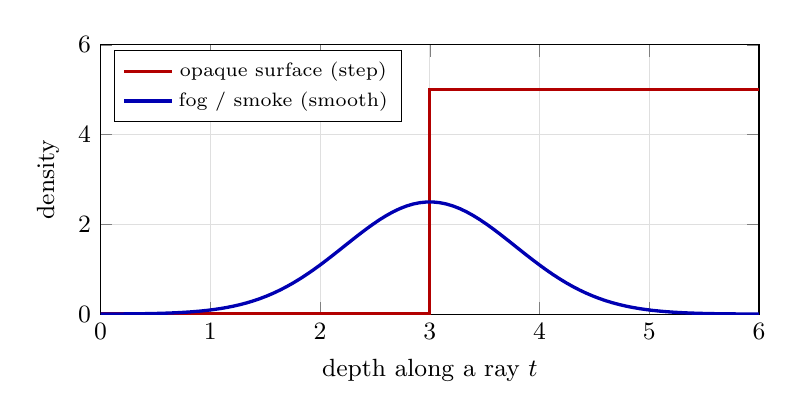
\begin{tikzpicture}
\begin{axis}[xlabel={depth along a ray $t$},ylabel={density},ymin=0,ymax=6,xmin=0,xmax=6,
  legend style={at={(0.02,0.98)},anchor=north west,font=\scriptsize},height=5cm]
 \addplot[very thick,red!70!black,const plot] coordinates {(0,0)(3,0)(3,5)(6,5)};
 \addlegendentry{opaque surface (step)}
 \addplot[very thick,blue!70!black,domain=0:6,samples=100] {2.5*exp(-((x-3)/1.1)^2)};
 \addlegendentry{fog / smoke (smooth)}
\end{axis}
\end{tikzpicture}
\caption{A surface is the limit of a density that rises from zero to ``very large'' in an infinitesimally thin layer.}\label{fig:density}
\end{figure}

\subsection{Density Fields\slides{10--11}}

\begin{definition}{Density field}{density}
A \emph{density field} (volume) is a non-negative function over space, either stored on a grid or defined continuously:
\[
V[x,y,z]\in\R^+ \quad (\text{discrete volume}),\qquad f(\mathbf p)\in\R^+ \quad (\text{continuous field},\ \mathbf p\in\R^3).
\]
\end{definition}

The slide shows smoke (a simulation) and a CT scan (a physical density map), and states \textbf{today's goal}: \emph{how do we render this representation?}

\photo{11}{NeRF objects (chair, Lego bulldozer, materials, drums, microphone, hotdog, ship, ficus). Figure credits: Mildenhall et al., ECCV 2020 (NeRF).}{6}

\begin{intuition}
A CT scan is the perfect mental model: each voxel stores ``how much X-ray gets absorbed here''. A camera is like an X-ray machine for \emph{visible light}: it needs to integrate something along each ray. Rendering = turning the 3D table of numbers into a 2D image.
\end{intuition}

%=====================================================================
\section{Sensor Physics\slides{12--16}}
%=====================================================================
Slide 12 introduces the question: \emph{how do radiance fields interact with a camera, and how are pixel colours formed?}

\subsection{Radiance\slides{13}}

\begin{definition}{Radiance (luminance)}{radiance}
\emph{Radiance} $L(\x,\w)$ is the photometric measure of the luminous intensity \emph{per unit area} of light travelling in a given direction $\w$ at the point $\x$ (more precisely: per unit area perpendicular to $\w$ and per unit solid angle $\dd\w$, see Fig.~\ref{fig:radiance}).
\end{definition}

\begin{figure}[h]
\centering
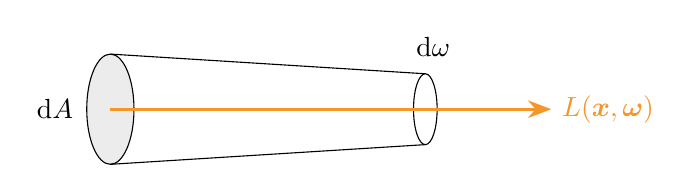
\begin{tikzpicture}[>=Stealth]
 \draw[fill=gray!15] (0,0) ellipse (0.3 and 0.7); \node[left] at (-0.35,0) {$\mathrm{d}A$};
 \draw (0,0.7)--(4,0.45); \draw (0,-0.7)--(4,-0.45);
 \draw[fill=white] (4,0) ellipse (0.15 and 0.45);
 \draw[->,very thick,orng] (0,0)--(5.6,0) node[right] {$L(\bm x,\bm\omega)$};
 \node[above] at (4.1,0.55) {$\mathrm{d}\omega$};
\end{tikzpicture}
\caption{Radiance: power flowing through an area element $\mathrm dA$ into a cone $\mathrm d\omega$ around direction $\bm\omega$. Figure idea: P.~Hanrahan.}\label{fig:radiance}
\end{figure}

\begin{intuition}
Radiance is ``what one pixel of a camera would measure''. Crucially it is \emph{constant along a ray in empty space} (a wall looks equally bright from 1~m or 5~m away). So a ray through vacuum carries one number per direction---that is what makes pixel $\leftrightarrow$ ray a clean correspondence. The whole lecture is about what happens to this number when the ray is \emph{not} in vacuum.
\end{intuition}

\subsection{Surface Rendering\slides{14}}

Let $\x^*$ be the optical centre and $\w$ the direction from $\x^*$ towards the sensor. For an opaque surface, the pixel value is proportional to the radiance emitted from the first surface point seen along the ray:
\[
\text{pixel}\;\propto\;L(\x^*,\w)\;=\;L(\x^*-\lambda\w,\;\w),
\]
where $\lambda>0$ is the distance to the surface along the ray.

\begin{intuition}
For surfaces the pixel is a \emph{single-point lookup}: find $\lambda$ (the depth!), evaluate the emitted radiance (shading, texture) at that point, done. This is why depth estimation was central in the previous lectures.
\end{intuition}

\subsection{A Ray Through a Medium\slides{15--16}}

If a medium (a cloud) sits between the surface and the camera, the equality breaks:
\[
\text{pixel}\;\propto\;L(\x^*,\w)\;\neq\;L(\x^*-\lambda\w,\;\w).
\]
The pixel value \emph{cannot} be reduced to the emitted radiance of a single surface point. Slide 16 phrases the new question:

\begin{center}\textbf{How does $L(\x,\w)$ vary along a ray?}\end{center}

\begin{figure}[h]
\centering
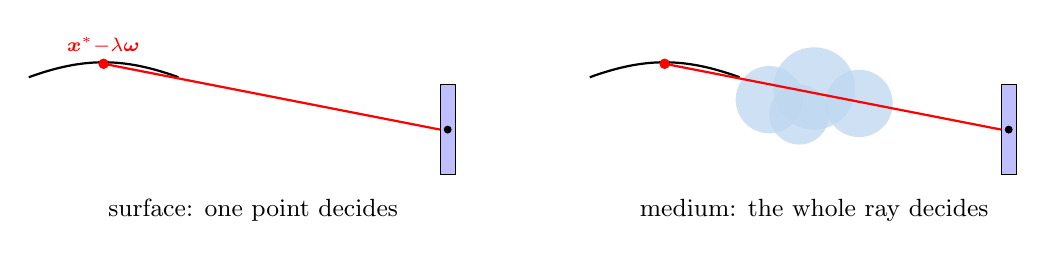
\begin{tikzpicture}[>=Stealth,scale=0.95]
 % left: surface
 \begin{scope}
  \draw[thick] (0,0.2) to[out=20,in=160] (2,0.2);
  \fill[red] (1,0.38) circle (2pt) node[above,font=\scriptsize] {$\bm x^*{-}\lambda\bm\omega$};
  \draw[red,thick] (1,0.38)--(5.5,-0.5);
  \draw[fill=blue!25] (5.5,-1.1) rectangle (5.7,0.1); \fill (5.6,-0.5) circle (1.5pt);
  \node[below] at (3,-1.3) {\small surface: one point decides};
 \end{scope}
 % right: medium
 \begin{scope}[xshift=7.5cm]
  \draw[thick] (0,0.2) to[out=20,in=160] (2,0.2);
  \fill[red] (1,0.38) circle (2pt);
  \foreach \cx/\cy/\r in {2.4/-0.1/0.45,3.0/0.05/0.55,3.6/-0.15/0.45,2.8/-0.3/0.4}
     \fill[cloud,opacity=0.75] (\cx,\cy) circle (\r);
  \draw[red,thick] (1,0.38)--(5.5,-0.5);
  \draw[fill=blue!25] (5.5,-1.1) rectangle (5.7,0.1); \fill (5.6,-0.5) circle (1.5pt);
  \node[below] at (3,-1.3) {\small medium: the whole ray decides};
 \end{scope}
\end{tikzpicture}
\caption{Surface rendering vs.\ rendering through a medium: the red ray accumulates the effect of everything it crosses.}
\end{figure}

%=====================================================================
\section{Volumetric Interactions\slides{17--24}}
%=====================================================================
Slide 17 introduces the next block: \emph{how different media perturb the luminance.} Light interacting with a medium can be absorbed, emitted, or scattered.

\subsection{Absorption\slides{18--19}}

Light travelling in a medium can get absorbed by it. Examples (slide 18): fog and dense black smoke. Slide 19 quotes Leonardo da Vinci's \emph{Treatise on Painting} (c.~1480): to make an object look five times as distant, paint it five times bluer---an early description of aerial perspective, i.e.\ distance-dependent attenuation.

\photo{18}{Absorption: fog and a smoke plume. Figure credits: I.~Gkioulekas.}{4.8}
\photo{19}{Absorption: da Vinci's self-portrait and \emph{Virgin of the Rocks} with the ``five times bluer'' quote (\emph{Treatise on Painting}, c.~1480). Figure credits: I.~Gkioulekas.}{5.5}

\begin{intuition}
The longer the path through the medium, the less of the original light survives; and since different wavelengths are attenuated differently, distant things shift colour (the blue haze in the paintings). This is the first hint of the exponential law we derive in Section~\ref{sec:finite}.
\end{intuition}

\subsection{What else?\slides{20}}

Light can also be \emph{added} by the medium.

\subsection{Emission\slides{21}}

Hot gases (explosions, flames) emit their own light along the ray.

\photo{21}{Emission: fireballs. Figure credits: I.~Gkioulekas.}{4.8}

\subsection{What else?\slides{22}}

Light shafts through a misty forest show something that is neither absorption nor emission.

\photo{22}{Light shafts through mist at sunrise (``What else?'').}{5}

\subsection{Scattering\slides{23}}

\emph{Light along a ray can depend on light in other directions.} In the atmosphere (slide figure) a sunbeam hits a molecule and is redirected towards the observer; rainbows are another example.

\photo{23}{Scattering: sun--atmosphere--observer sketch and a double rainbow. Figure credits: I.~Gkioulekas.}{5}

\subsection{Volume Rendering a Ray\slides{24}}

\begin{center}\textbf{How does $L(\x,\w)$ vary along a ray?}\quad Emission, absorption and scattering.\end{center}

The following figure summarises the four elementary mechanisms (they are formalised in the next section).

\begin{figure}[h]
\centering
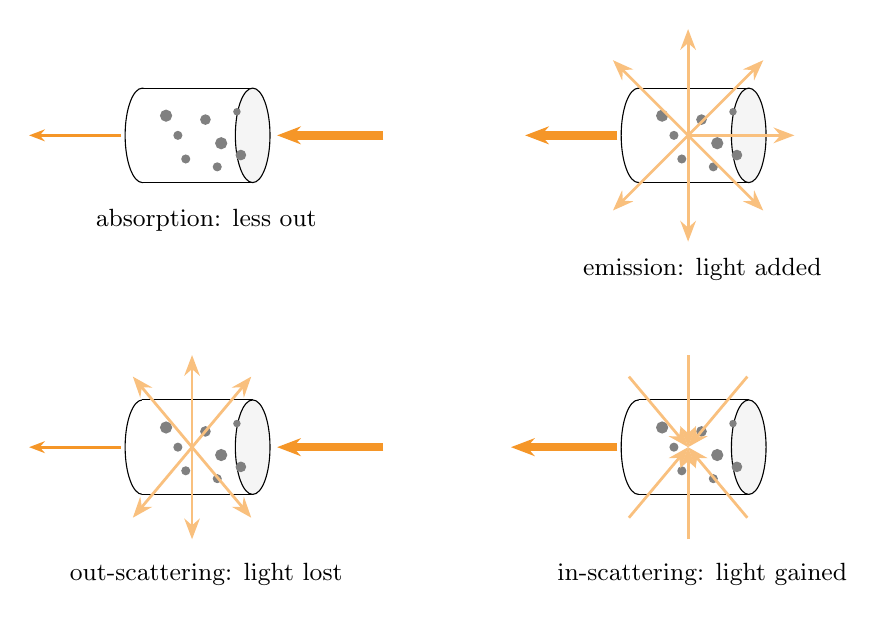
\begin{tikzpicture}[>=Stealth,scale=0.9]
 \tikzset{big/.style={-{Stealth[length=3mm]},line width=3pt,orng},
          thin_/.style={-{Stealth[length=2mm]},line width=1pt,orng},
          rad/.style={-{Stealth},line width=1pt,orng!60}}
 % absorption
 \begin{scope}
  \pic at (0,0) {slab};
  \draw[big] (3.4,0)--(1.9,0); \draw[thin_] (-0.3,0)--(-1.6,0);
  \node[below] at (0.9,-0.9) {\small absorption: less out};
 \end{scope}
 % emission
 \begin{scope}[xshift=7cm]
  \pic at (0,0) {slab};
  \foreach \a in {45,90,135,225,270,315,0} \draw[rad] (0.7,0) -- ++(\a:1.5);
  \draw[big] (-0.3,0)--(-1.6,0);
  \node[below] at (0.9,-1.6) {\small emission: light added};
 \end{scope}
 % out-scattering
 \begin{scope}[yshift=-4.4cm]
  \pic at (0,0) {slab};
  \draw[big] (3.4,0)--(1.9,0); \draw[thin_] (-0.3,0)--(-1.6,0);
  \foreach \a in {50,90,130,230,270,310} \draw[rad] (0.7,0) -- ++(\a:1.3);
  \node[below] at (0.9,-1.5) {\small out-scattering: light lost};
 \end{scope}
 % in-scattering
 \begin{scope}[xshift=7cm,yshift=-4.4cm]
  \pic at (0,0) {slab};
  \foreach \a in {50,90,130,230,270,310} \draw[rad] ($(0.7,0)+(\a:1.3)$) -- (0.7,0);
  \draw[big] (-0.3,0)--(-1.8,0);
  \node[below] at (0.9,-1.5) {\small in-scattering: light gained};
 \end{scope}
\end{tikzpicture}
\caption{Interactions of light with a small cylinder of medium (thick orange = strong radiance, thin = weak).}\label{fig:four}
\end{figure}

%=====================================================================
\section{Dissecting Volume Rendering\slides{25--39}}
%=====================================================================
\textbf{Today's goals (slide 25).} (1) Mathematical models of emission and absorption; (2) the volume rendering equation and transmittance; (3) computational algorithms for volume rendering; (4) next lecture: combine with neural representations.

\subsection{Volume Rendering a Ray\slides{26}}

Consider a thin cylinder of medium, cross-section $\mathrm dA$ and length $z$, with the camera at one end. The slide asks: \emph{how much light is lost or gained along the differential beam because of the interactions of light with the medium?} We study an \emph{infinitesimal} slice of length $\mathrm dz$ and later integrate.

\subsection{Volume Rendering a Ray: Absorption\slides{27--28}}

\begin{definition}{Absorption coefficient}{abs}
The \emph{absorption coefficient} $\sigma_a(\x)\ge 0$ (units: length$^{-1}$) is the fraction of radiance absorbed per unit length at $\x$:
\[
\mathrm dL(\x,\w)\;=\;-\sigma_a(\x)\,L(\x,\w)\,\mathrm dz .
\]
\end{definition}

\subsubsection*{Simple derivation of the absorption equation (slide 28)}
Assume the slice of length $\mathrm dz$ contains opaque spherical particles of radius $r$ in empty space, with $\rho$ particles per unit volume (Fig.~\ref{fig:particles}).

\begin{figure}[h]
\centering
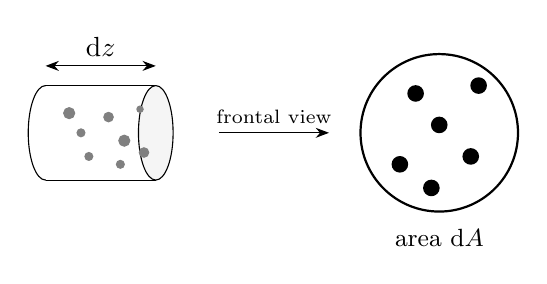
\begin{tikzpicture}[>=Stealth]
 \pic at (0,0) {slab};
 \draw[<->] (0,0.85)--(1.4,0.85) node[midway,above] {$\mathrm dz$};
 \draw[->] (2.2,0)--(3.6,0) node[midway,above,font=\scriptsize] {frontal view};
 \draw[thick] (5,0) circle (1);
 \foreach \px/\py in {-0.3/0.5,0.4/-0.3,0.5/0.6,-0.5/-0.4,0.0/0.1,-0.1/-0.7} \fill (5+\px,\py) circle (3pt);
 \node[below] at (5,-1.1) {\small area $\mathrm dA$};
\end{tikzpicture}
\caption{Opaque particles seen along the beam: each blocks a disc of area $\pi r^2$.}\label{fig:particles}
\end{figure}

\begin{lemma}{Absorption by opaque particles}{particles}
Let $f$ be the fraction of the cross-section $\mathrm dA$ covered by particles in the slice. Then $f=\rho\pi r^2\,\mathrm dz$, $L_o=(1-f)L_i$ and therefore
\[
\mathrm dL=L_o-L_i=-fL_i=-(\rho\pi r^2)\,L\,\mathrm dz=-\sigma_aL\,\mathrm dz,\qquad \sigma_a=\rho\pi r^2 .
\]
\end{lemma}
\begin{proof}
The slice contains $\rho\,\mathrm dA\,\mathrm dz$ particles, each hiding area $\pi r^2$ (assuming $\mathrm dz$ so small that discs do not overlap in the frontal view). The covered fraction is $f=(\rho\,\mathrm dA\,\mathrm dz)\,\pi r^2/\mathrm dA=\rho\pi r^2\mathrm dz$. Only the uncovered fraction $1-f$ of the incoming radiance $L_i$ gets through.
\end{proof}

\begin{intuition}
$\sigma_a=\rho\cdot\pi r^2$ is \emph{(how many particles per volume) $\times$ (how big a shadow each casts)}: denser or bigger particles $\Rightarrow$ larger $\sigma_a$. Worked number: if $\sigma_a=0.5\,\mathrm{m^{-1}}$ then a slice of $\mathrm dz=1\,\mathrm{cm}$ removes $0.5\cdot0.01=0.5\%$ of the light. Tiny per slice, but a ray crosses many slices (that is what the integral of Section~\ref{sec:finite} does).
\end{intuition}

\subsection{Volume Rendering a Ray: Emission\slides{29}}

\begin{definition}{Emission term}{emission}
Let $L_e(\x,\w)$ be the radiance emitted by the medium at $\x$ in direction $\w$. The gain along a slice is
\[
\mathrm dL(\x,\w)=\sigma_a(\x)\,L_e(\x,\w)\,\mathrm dz .
\]
\end{definition}

\begin{intuition}
Note the factor $\sigma_a$: emission is weighted by the same coefficient as absorption. Where there is no matter ($\sigma_a=0$) nothing can glow; where there is a lot, the glow is strong. It also makes the convention ``$L_e$ is the colour of the stuff, $\sigma_a$ is how much stuff'' very natural, which is exactly how NeRF splits its outputs (colour and density).
\end{intuition}

\subsection{Emission-Absorption Model\slides{30}}

Putting the two together:
\[
\mathrm dL(\x,\w)=\underbrace{-\sigma_a(\x)L(\x,\w)\mathrm dz}_{\text{losses}}\;+\;\underbrace{\sigma_a(\x)L_e(\x,\w)\mathrm dz}_{\text{gains}} .
\]

\subsection{The Out-Scattering Term\slides{31}}

\begin{definition}{Scattering coefficient, out-scattering}{outscat}
Light can be deflected away from the ray. With the \emph{scattering coefficient} $\sigma_s(\x)$:
\[
\mathrm dL(\x,\w)=-\sigma_s(\x)\,L(\x,\w)\,\mathrm dz .
\]
\end{definition}
It is mathematically identical to absorption (a loss proportional to the incident radiance); the only difference is where the lost energy goes: absorption turns it into heat, out-scattering sends it into other directions.

\subsection{The In-Scattering Term\slides{32--33}}

\begin{definition}{In-scattering and phase function}{inscat}
Light coming from other directions $\w'$ can be redirected into the ray direction $\w$:
\[
\mathrm dL(\x,\w)=\sigma_s(\x)\,L_s(\x,\w)\,\mathrm dz,\qquad
L_s(\x_t,\w)=\int_{\Sph}f_p(\x_t,\w',\w)\,L_i(\x_t,\w')\dd\w' .
\]
Here $f_p$ is the \emph{phase function} (the probability density that light arriving from $\w'$ leaves towards $\w$; by the usual convention it integrates to one over $\w$, which is not stated on the slide).
\end{definition}

The slide's warning: \emph{unfortunately $L_s$ is non-trivial}, and ``$L_i$ can also depend on other scattered light!''.

\begin{intuition}
To know the light along \emph{this} ray, I need the light along \emph{all} rays through the point $\x_t$ (a sphere of directions). But each of those rays has the same problem, and so on: the unknown $L$ appears on both sides of the equation, inside an integral over a sphere, recursively. That is why full scattering is expensive (Monte-Carlo path tracing in graphics), and why the next section asks whether we can live without it.
\end{intuition}

\subsection{The Radiative Transfer Equation\slides{34}}

\begin{theorem}{Radiative transfer equation (RTE)}{rte}
Collecting the four mechanisms,
\[
\mathrm dL(\x,\w)=\underbrace{-\sigma_a(\x)L(\x,\w)\mathrm dz-\sigma_s(\x)L(\x,\w)\mathrm dz}_{\text{losses: absorption, out-scattering}}
+\underbrace{\sigma_a(\x)L_e(\x,\w)\mathrm dz+\sigma_s(\x)L_s(\x,\w)\mathrm dz}_{\text{gains: emission, in-scattering}} .
\]
\end{theorem}

\begin{intuition}
Four knobs, two losses and two gains, exactly the panels of Fig.~\ref{fig:four}. It is the ``energy bookkeeping'' of a beam crossing a small piece of fog.
\end{intuition}

\subsection{The Emission-Absorption Model\slides{35--36}}

Slide 35 is the section divider \emph{``7.5 The Emission-Absorption Model: do we really need scattering?''}. Slide 36 ``drops scattering'' (the grayed terms) and keeps only
\[
\mathrm dL(\x,\w)=-\sigma_a(\x)L(\x,\w)\mathrm dz+\sigma_a(\x)L_e(\x,\w)\mathrm dz ,
\]
noting that this is \textbf{the de-facto standard in neural volume rendering methods}. The slide then asks: \emph{isn't this too restrictive?}

\subsection{Expressivity of the EA Model\slides{37}}

The answer is: \emph{not under an arbitrarily allowed $L_e'$}.

\begin{proposition}{Scattering can be absorbed into the emission term}{expr}
Define the \emph{effective emission}
\[
L_e'=L_e+\frac{\sigma_s}{\sigma_a}\,(L_s-L).
\]
Then the full RTE of Theorem~\ref{thm:rte} is a pure emission--absorption equation with absorption coefficient $\sigma_a$ and emission $L_e'$:
$\mathrm dL=-\sigma_aL\,\mathrm dz+\sigma_aL_e'\,\mathrm dz$.
\end{proposition}
\begin{proof}
Factor $\sigma_a$ out of the four terms:
$-\sigma_aL-\sigma_sL+\sigma_aL_e+\sigma_sL_s=-\sigma_aL+\sigma_a\bigl[L_e+\tfrac{\sigma_s}{\sigma_a}(L_s-L)\bigr]$.
\end{proof}

\begin{intuition}
A learner that is free to output \emph{any} colour at each point and for each viewing direction can mimic scattering: whatever scattering would add or remove at a point is simply baked into the colour it outputs there. The catch: $L_e'$ now depends on $L$, $L_s$ and the viewing direction, so it is a complicated function---it needs a flexible (neural) colour model, and the learned colour will not be physically \emph{relightable}. This is the bridge to NeRF, where the colour network takes the view direction as input.
\end{intuition}

\subsection{Why Model Scattering at All\slides{38}}

Simple scenes with a more ``complete'' rendering model can produce interesting effects (slide: two glasses of translucent liquid with glowing edges), whereas one would need complex, inhomogeneous scenes to reproduce them in an EA model. Scattering models also allow \textbf{relighting}, which is the focus of lesson 11.

\photo{38}{Two glasses of translucent liquid rendered with scattering. Figure credits: I.~Gkioulekas.}{5.2}

\subsection{Notation From Here On\slides{39}}

From now on we drop the subscript: $\sigma_a\equiv\sigma$, and we work with
\[
\mathrm dL(\x,\w)=-\sigma(\x)\,L(\x,\w)\mathrm dz+\sigma(\x)\,L_e(\x,\w)\mathrm dz .
\]

%=====================================================================
\section{From Infinitesimal to Finite Lengths\slides{40--54}}\label{sec:finite}
%=====================================================================
Slide 40 is the divider ``7.6 From Infinitesimal to Finite Lengths''.

\subsection{From infinitesimal to finite lengths\slides{41}}

The plan: (1) model the \emph{absorption-only} case; (2) then allow emission.

\subsection{Absorption-only Volume Rendering\slides{42}}

For a \emph{homogeneous} medium (uniform density $\sigma$), $\mathrm dL=-\sigma L\,\mathrm dz$.

\begin{proposition}{Beer--Lambert law}{beer}
In a homogeneous absorbing medium, light travelling a distance $z$ is attenuated exponentially:
\[
L(\x_0+\w z,\w)=e^{-\sigma z}\,L(\x_0,\w).
\]
\end{proposition}
\begin{proof}
Along the ray, $\ell(z):=L(\x_0+\w z,\w)$ satisfies $\ell'(z)=-\sigma\ell(z)$, a linear ODE with solution $\ell(z)=\ell(0)e^{-\sigma z}$.
\end{proof}

\begin{intuition}
Per unit length a fixed \emph{fraction} of the surviving light is removed, so the loss compounds like interest at rate $\sigma$. Numbers: with $\sigma=0.5\,\mathrm m^{-1}$, after 2~m only $e^{-1}\approx 37\%$ survives, after 6~m only $e^{-3}\approx5\%$.
\end{intuition}

\subsection{Absorption Only, Heterogeneous Medium\slides{43}}

If $\sigma$ varies in space, $\mathrm dL=-\sigma(\x)L\,\mathrm dz$ is still solvable.

\begin{definition}{Transmittance}{transm}
For two points $\x,\y$, let $\w_{xy}=(\y-\x)/\|\y-\x\|$. The \emph{transmittance}
\[
T(\x,\y)=\exp\!\Bigl(-\!\int_{t=0}^{\|\x-\y\|}\sigma(\x+\w_{xy}t)\dd t\Bigr)
\]
is the fraction of the radiance leaving $\x$ towards $\y$ that reaches $\y$ along a straight line, under the absorption-only model. For a homogeneous medium $T(\x,\y)=e^{-\sigma\|\x-\y\|}$.
\end{definition}

\begin{proposition}{Absorption-only solution, heterogeneous medium}{hetero}
$L(\x_0+\w z,\w)=T(\x_0,\x_0+\w z)\,L(\x_0,\w)$, i.e.\ $L(\x_0+\w z,\w)=e^{-\int_0^z\sigma(\x_0+\w t)\mathrm dt}L(\x_0,\w)$.
\end{proposition}
\begin{proof}
Let $\ell(s)=L(\x_0+\w s,\w)$ and $\tau(s)=\int_0^s\sigma(\x_0+\w t)\mathrm dt$ (the \emph{optical depth}). The ODE is $\ell'=-\sigma\ell$. Then $\frac{\mathrm d}{\mathrm ds}\bigl(e^{\tau(s)}\ell(s)\bigr)=e^{\tau}(\sigma\ell+\ell')=0$, so $e^{\tau(z)}\ell(z)=\ell(0)$.
\end{proof}

\begin{intuition}
The integral $\tau=\int\sigma$ simply \emph{adds up the opacity met along the way}; the exponential converts that total into a surviving fraction. It does not matter \emph{where} the dense bits are, only their total: a thin dense slab and a long thin haze with equal $\int\sigma$ dim the light equally.
\end{intuition}

\subsection{Transmittance\slides{44--45}}

\begin{lemma}{Multiplicativity}{mult}
For $\z$ on the segment between $\x$ and $\y$: $T(\x,\y)=T(\x,\z)\,T(\z,\y)$.
\end{lemma}
\begin{proof}
The integral of $\sigma$ over a segment is additive over its two sub-segments, and $e^{a+b}=e^ae^b$.
\end{proof}

\begin{lemma}{Symmetry (the slide-44 question)}{sym}
$T(\x,\y)=T(\y,\x)$.
\end{lemma}
\begin{proof}
Both are $\exp(-\int\sigma)$ over the \emph{same} segment; reversing the parametrisation $t\mapsto\|\x-\y\|-t$ does not change the value of the integral.
\end{proof}

\begin{intuition}
Transmittance only depends on how much stuff lies \emph{between} two points, not on which way the light travels. Think of a pane of tinted glass: it dims light by the same factor in either direction. (Symmetry would fail only if the medium itself depended on the direction of travel, which is not the case here.)
\end{intuition}

\begin{figure}[h]
\centering
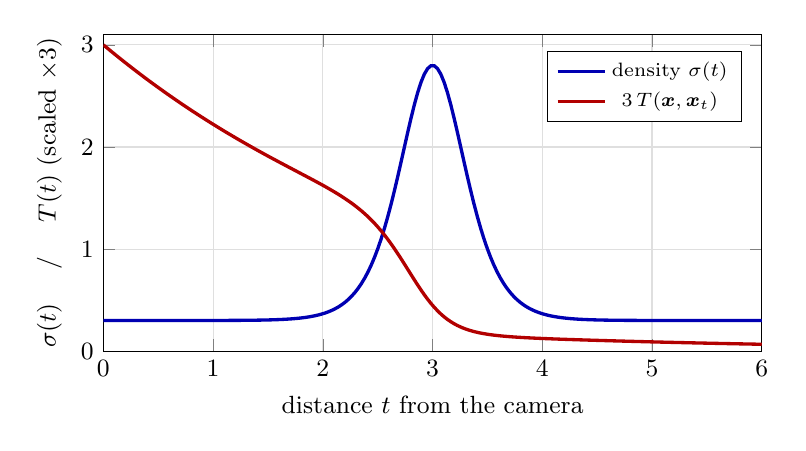
\begin{tikzpicture}
\begin{axis}[xlabel={distance $t$ from the camera},xmin=0,xmax=6,ymin=0,ymax=3.1,
  ytick={0,1,2,3},legend style={at={(0.97,0.95)},anchor=north east,font=\scriptsize},
  ylabel={$\sigma(t)$ \quad / \quad $T(t)$ (scaled $\times3$)}]
 \addplot[very thick,blue!70!black,domain=0:6,samples=200] {0.3+2.5/(cosh((x-3)/0.4))^2};
 \addlegendentry{density $\sigma(t)$}
 \addplot[very thick,red!70!black,domain=0:6,samples=200] {3*exp(-(0.3*x+tanh((x-3)/0.4)+1))};
 \addlegendentry{$3\,T(\bm x,\bm x_t)$}
\end{axis}
\end{tikzpicture}
\caption{Transmittance along a ray through a medium with a dense layer at $t=3$ (here $\sigma(t)=0.3+2.5\,\mathrm{sech}^2\frac{t-3}{0.4}$, so $\tau(t)=0.3t+\tanh\frac{t-3}{0.4}+1$ exactly). $T$ decays slowly in the haze and drops steeply across the dense layer; compare with slide 44.}
\end{figure}

\subsection{Absorption-only Volume Rendering\slides{46--48}}

Let $\x_z$ be a point behind the medium (e.g.\ a wall) and $\x$ the camera.

\begin{corollary}{Absorption-only rendering}{absrender}
$L(\x,\w)=T(\x,\x_z)\,L(\x_z,\w)$: the light reaching $\x$ is the light emitted at $\x_z$ modulated by the transmittance $T(\x,\x_z)$.
\end{corollary}

This is the radiance from ``outside'' the medium (slide 48). Slide 47 shows typical absorption-only media: whisky glasses and fog.

\photo{47}{Absorption-only media: tinted glass liquid and fog. Figure credits: I.~Gkioulekas.}{4.8}

\subsection{Adding Emission\slides{49}}

Now let the medium also emit, with $\x_t=\x-t\w$ the point at depth $t$ along the ray from the camera and $\x_z$ the background point at depth $z$.

\begin{theorem}{Emission--absorption volume rendering equation}{vre}
\[
L(\x,\w)=\underbrace{T(\x,\x_z)\,L(\x_z,\w)}_{\text{background (outside)}}+\underbrace{\int_0^zT(\x,\x_t)\,\sigma(\x_t)\,L_e(\x_t,\w)\dd t}_{\text{accumulated emission from inside}} .
\]
\end{theorem}
\begin{proof}
Let $\ell(t)=L(\x_t,\w)$ be the radiance at depth $t$. Light travels towards the camera, i.e.\ towards \emph{decreasing} $t$, so $\mathrm dz=-\mathrm dt$ in the slide's ODE and
$\ell'(t)=\sigma(\x_t)\,\ell(t)-\sigma(\x_t)\,L_e(\x_t,\w)$. With $\tau(t)=\int_0^t\sigma(\x_s)\mathrm ds$ and $T(\x,\x_t)=e^{-\tau(t)}$:
\[
\frac{\mathrm d}{\mathrm dt}\bigl(e^{-\tau(t)}\ell(t)\bigr)=e^{-\tau}(\ell'-\sigma\ell)=-\sigma(\x_t)\,e^{-\tau(t)}L_e(\x_t,\w).
\]
Integrate from $0$ to $z$: $e^{-\tau(z)}\ell(z)-\ell(0)=-\int_0^z\sigma\,e^{-\tau}L_e\,\mathrm dt$. Since $\ell(0)=L(\x,\w)$ and $\ell(z)=L(\x_z,\w)$, rearranging gives the claim.
\end{proof}

\begin{intuition}
Every point along the ray ``shouts'' with loudness $\sigma(\x_t)L_e(\x_t,\w)$ (how much matter $\times$ how bright it is). Its shout then travels to the camera and is attenuated by everything in between, $T(\x,\x_t)$. The pixel is the sum of all shouts plus the muffled background. \emph{Points closer to the camera are less muffled}, which is exactly why near stuff occludes far stuff without any explicit visibility test.
\end{intuition}

\subsection{Emission-Absorption Volume Rendering\slides{50}}

Slide 50 repeats the equation and asks: \emph{can we compute this analytically? Approximately?} The next slides answer: analytically only in special cases, approximately in general.

\subsection{Special Case: Homogeneous, Non-Emitting Medium\slides{51}}

With $L_e\equiv0$ and constant $\sigma$ the integral vanishes, $T(\x,\x_z)=e^{-\sigma\Delta}$ and
\[
L(\x,\w)=e^{-\sigma\Delta}L(\x_z,\w),
\]
where $\Delta$ is the distance travelled in the medium: the inner term depends only on $\Delta$.

\subsection{Special Case: Homogeneous emitting medium\slides{52--53}}

\begin{lemma}{Homogeneous emitting segment}{homog}
Let $\sigma$ and $L_e(\x,\w)\equiv C$ be constant on a segment of length $\Delta$ (depth $\delta$ measured from the camera side). Then
\[
L(\x,\w)=e^{-\sigma\Delta}L(\x_z,\w)+\bigl(1-e^{-\sigma\Delta}\bigr)C .
\]
In particular the emission of the segment alone is $\bigl(1-e^{-\sigma\Delta}\bigr)C$.
\end{lemma}
\begin{proof}
By Theorem~\ref{thm:vre}, the emission integral is $\int_0^\Delta e^{-\sigma\delta}\sigma C\,\mathrm d\delta=C\bigl[-e^{-\sigma\delta}\bigr]_0^\Delta=C(1-e^{-\sigma\Delta})$.
\end{proof}

\begin{remark}
Slide 53 writes the antiderivative as $\int\lambda e^{-\lambda x}\mathrm dx=-e^{\lambda x}+c$; the correct primitive is $-e^{-\lambda x}+c$, which is what the computation above uses.
\end{remark}

\begin{intuition}
The result is a \emph{convex blend}: weight $e^{-\sigma\Delta}$ on what is behind and weight $1-e^{-\sigma\Delta}$ on the colour of the medium. It is precisely \emph{alpha blending} with opacity $\alpha=1-e^{-\sigma\Delta}$. Numbers for $\sigma=0.5\,\mathrm m^{-1}$, $\Delta=2$~m: $\alpha=1-e^{-1}\approx0.63$, so the pixel is $37\%$ background and $63\%$ medium colour. As $\Delta\to\infty$ the medium becomes opaque and the background disappears (Fig.~\ref{fig:alpha}), so a thick-enough volume behaves like a surface.
\end{intuition}

\begin{figure}[h]
\centering
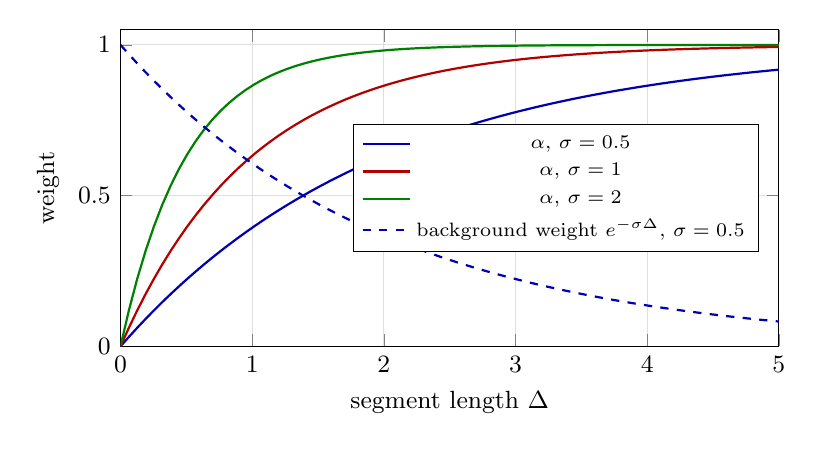
\begin{tikzpicture}
\begin{axis}[xlabel={segment length $\Delta$},ylabel={weight},xmin=0,xmax=5,ymin=0,ymax=1.05,
  legend style={at={(0.97,0.5)},anchor=east,font=\scriptsize}]
 \addplot[thick,blue!70!black,domain=0:5,samples=80] {1-exp(-0.5*x)}; \addlegendentry{$\alpha$, $\sigma=0.5$}
 \addplot[thick,red!70!black,domain=0:5,samples=80] {1-exp(-1*x)}; \addlegendentry{$\alpha$, $\sigma=1$}
 \addplot[thick,green!50!black,domain=0:5,samples=80] {1-exp(-2*x)}; \addlegendentry{$\alpha$, $\sigma=2$}
 \addplot[thick,dashed,blue!70!black,domain=0:5,samples=80] {exp(-0.5*x)}; \addlegendentry{background weight $e^{-\sigma\Delta}$, $\sigma=0.5$}
\end{axis}
\end{tikzpicture}
\caption{Opacity $\alpha=1-e^{-\sigma\Delta}$ of a homogeneous segment and (dashed) the fraction of background that survives, for different densities.}\label{fig:alpha}
\end{figure}

\subsection{What Can We Render?\slides{54}}

Slide 54 contrasts what is within reach and what is not. Within reach (\checkmark): homogeneous EA media such as fog and mist-covered landscapes. Out of reach ($\times$) for the homogeneous EA special case: smoke plumes with fire, light shafts, jade, rainbows, whisky.

\photo{54}{What can we render? Homogeneous EA (fog, misty scenery) vs.\ out of reach (smoke, light shafts, jade, rainbow, whisky). Figure credits: I.~Gkioulekas.}{6}

\begin{intuition}
The closed forms above are lovely but only apply to uniform media. For anything with structure (a smoke plume, a learned density field) $\sigma$ and $L_e$ vary along the ray, and we need numerics.
\end{intuition}

%=====================================================================
\section{Computational Volume Rendering\slides{55--68}}
%=====================================================================
\subsection{Computational Volume Rendering\slides{56--57}}

In the general case (spatially varying coefficient and/or emission) there is \textbf{no analytical solution} to the equation of Theorem~\ref{thm:vre}. To simplify, slide 57 first \emph{ignores the light from outside the medium}:
\[
L(\x,\w)=\int_0^zT(\x,\x_t)\,\sigma(\x_t)\,L_e(\x_t,\w)\dd t .
\]
The background term is reinstated at slide 67.

\subsection{Ray Marching\slides{58--63}}

Approximate the integral with a discrete sum. Place samples $\x_{t_1},\dots,\x_{t_{N+1}}$ along the ray (with $t_1=0$), so there are $N$ segments with $\Delta_t$ the distance between successive samples (slide 58: ``$\x_{t_i}$ is the $i^{\mathrm{th}}$ sample along the ray at depth $t_i$'').

\begin{figure}[h]
\centering
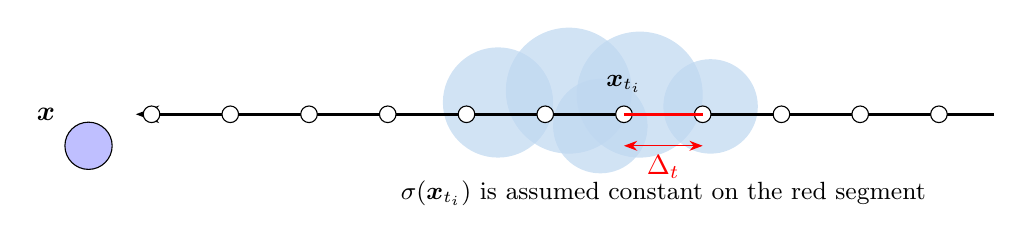
\begin{tikzpicture}[>=Stealth]
 \foreach \cx/\cy/\r in {5.2/0.15/0.7,6.1/0.3/0.8,7.0/0.25/0.8,7.9/0.1/0.6,6.5/-0.15/0.6}
     \fill[cloud,opacity=0.7] (\cx,\cy) circle (\r);
 \draw[->,very thick] (11.5,0)--(0.6,0);
 \draw[fill=blue!25] (0,-0.4) circle (0.3); \node[left] at (-0.3,0) {$\bm x$};
 \foreach \i in {1,...,11} \draw[fill=white] ({0.8+\i-1},0) circle (3pt);
 \draw[red,very thick] (6.8,0)--(7.8,0);
 \node[above,font=\small] at (6.8,0.15) {$\bm x_{t_i}$};
 \draw[<->,red] (6.8,-0.4)--(7.8,-0.4) node[midway,below] {$\Delta_t$};
 \node[font=\small] at (7.3,-1.0) {$\sigma(\bm x_{t_i})$ is assumed constant on the red segment};
\end{tikzpicture}
\caption{Ray marching: samples along the ray, each representing the segment that follows it.}\label{fig:march}
\end{figure}

\subsubsection*{Step 1: contribution of segment $i$}
Slide 59 writes $L(\x,\w)\approx\sum_{i=1}^NT(\x,\x_{t_i})\times(\text{emission from the }i^{\mathrm{th}}\text{ segment})$, and slide 60 fills in the emission using Lemma~\ref{lem:homog} under the assumption that the medium is homogeneous within $\Delta_t$:

\begin{proposition}{Ray-marching approximation}{march}
Assume $\sigma\equiv\sigma_{t_i}$ and $L_e\equiv L_e(\x_{t_i},\w)$ on segment $i$. Then
\[
L(\x,\w)\approx\sum_{i=1}^{N}T(\x,\x_{t_i})\,\bigl(1-e^{-\sigma_{t_i}\Delta_t}\bigr)\,L_e(\x_{t_i},\w)
\]
with
\[
T(\x,\x_{t_i})=T(\x,\x_{t_{i-1}})\,e^{-\sigma_{t_{i-1}}\Delta_t},\quad T(\x,\x_{t_1})=1.
\]
\end{proposition}
\begin{proof}
Split the integral of Theorem~\ref{thm:vre} (without background) over the segments. For $t\in[t_i,t_i+\Delta_t]$, multiplicativity (Lemma~\ref{lem:mult}) gives $T(\x,\x_t)=T(\x,\x_{t_i})\,e^{-\sigma_{t_i}(t-t_i)}$, so segment $i$ contributes $T(\x,\x_{t_i})\int_0^{\Delta_t}e^{-\sigma_{t_i}\delta}\sigma_{t_i}L_e\mathrm d\delta=T(\x,\x_{t_i})(1-e^{-\sigma_{t_i}\Delta_t})L_e$ by Lemma~\ref{lem:homog}. The recursion for $T$ is multiplicativity applied to the $(i-1)$-th segment, using $T(\x_{t_{i-1}},\x_{t_i})=e^{-\sigma_{t_{i-1}}\Delta_t}$ (homogeneous within the segment); the base case is that the camera sits at the first sample.
\end{proof}

\begin{remark}
Slide 68 writes the recursion with $e^{+\sigma_{t_{i-1}}\Delta_t}$; the minus sign (as on slides 61 and 65) is the correct one: transmittance can only decrease along the ray.
\end{remark}

\begin{definition}{Opacity and weight of a sample}{alpha}
Let $\alpha_i=1-e^{-\sigma_{t_i}\Delta_t}$ (opacity of segment $i$), $T_i=T(\x,\x_{t_i})=\prod_{j<i}(1-\alpha_j)$ and $w_i=T_i\alpha_i$. Then $L\approx\sum_iw_i\,L_e(\x_{t_i},\w)$.
\end{definition}

\begin{intuition}
This is front-to-back \emph{alpha compositing}, the classic ``over'' operator. Walk away from the camera: each sample adds a fraction $\alpha_i$ of its colour, multiplied by the fraction $T_i$ of the ray that is still ``unspent''. For small steps $\alpha_i\approx\sigma_{t_i}\Delta_t$, which is the plain Riemann sum of the integral; the exponential form is better because it stays in $[0,1]$ even for huge $\sigma$ or large steps.
\end{intuition}

\begin{proposition}{Weights form a partition of unity}{unity}
(\emph{Not on the slides.}) With $T_{N+1}=\prod_{i=1}^N(1-\alpha_i)$, we have $\sum_{i=1}^Nw_i=1-T_{N+1}$. So $\sum_iw_i\le1$ and the leftover $T_{N+1}$ is exactly the weight left for the background, as on slide 67.
\end{proposition}
\begin{proof}
$w_i=T_i\alpha_i=T_i-T_i(1-\alpha_i)=T_i-T_{i+1}$, so the sum telescopes to $T_1-T_{N+1}=1-T_{N+1}$.
\end{proof}

\begin{intuition}
Think of the ray as carrying one unit of ``attention''. Each sample takes a share $w_i$ and hands the rest on. If the medium is dense, the shares are used up before the end and nothing is left for the background, while in thin media $T_{N+1}$ stays close to 1 and the background shows through. This is also why the same formulas make opaque objects: a very large $\sigma_{t_i}$ gives $\alpha_i\to1$ and $w_i\to T_i$, all remaining attention goes to \emph{that} sample, a surface.
\end{intuition}

\begin{algorithm}{Ray marching with uniform samples (slide 62--63)}{uniform}
\begin{algorithmic}[1]
\State \textbf{Input:} ray origin $\x$, direction $\bm d$, volume with $\sigma(\cdot)$ and colour $c(\cdot)$, $n$ samples, max range $t_{\max}$
\State $T\gets1$, \quad $C\gets0$, \quad $\Delta_t\gets t_{\max}/n$, \quad $t\gets0$
\While{$t<t_{\max}$}
 \State $\bm p\gets\x+\bm d\,t$;\quad $(\sigma,c)\gets\text{volume}(\bm p)$
 \State $\alpha\gets1-\exp(-\sigma\Delta_t)$ \Comment{opacity of this segment}
 \State $C\gets C+T\,\alpha\,c$
 \State $T\gets T\exp(-\sigma\Delta_t)$ \Comment{multiplicativity}
 \State $t\gets t+\Delta_t$
\EndWhile
\State \Return $C$
\end{algorithmic}
\end{algorithm}

The slide's Python (verbatim in spirit):
\begin{lstlisting}[language=Python,basicstyle=\ttfamily\footnotesize,frame=single,numbers=left,numberstyle=\tiny]
def raymarch_uniform(x, d, vol, n_samples, max_range):
    T = 1
    color = Color(0, 0, 0)
    delta_t = max_range / n_samples    # same step everywhere
    t = 0
    while t < max_range:
        p = x + d * t
        sigma, c = vol.at(p).density, vol.at(p).color
        alpha = 1 - exp(-sigma * delta_t)  # opacity of this segment
        color += T * alpha * c
        T *= exp(-sigma * delta_t)         # multiplicativity
        t += delta_t
    return color
\end{lstlisting}

\begin{example}{A three-sample ray}{three}
(\emph{Worked numbers, not on the slides.}) Let $\Delta_t=0.5$, $\sigma=(0.4,\,2.0,\,4.0)$ and scalar colours $c=(0.2,\,0.8,\,1.0)$, no background. Then
$\alpha=(1-e^{-0.2},\,1-e^{-1},\,1-e^{-2})=(0.181,\,0.632,\,0.865)$, $T=(1,\;0.819,\;0.301)$, $T_4=0.041$, and
$w=T\alpha=(0.181,\,0.518,\,0.260)$.
Check: $\sum w_i=0.959=1-T_4$. The pixel is $0.181\cdot0.2+0.518\cdot0.8+0.260\cdot1.0\approx0.711$. With a background of radiance $0.5$ one adds $T_4\cdot0.5\approx0.020$, giving $0.731$.
\end{example}

\begin{figure}[h]
\centering
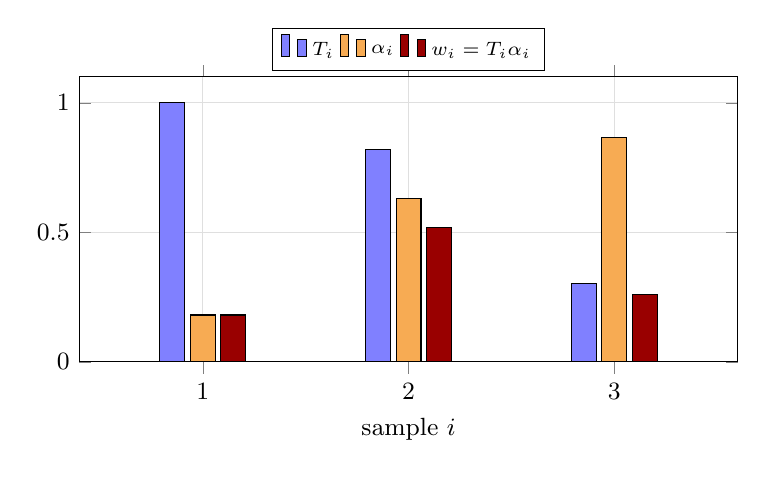
\begin{tikzpicture}
\begin{axis}[ybar,bar width=9pt,xlabel={sample $i$},symbolic x coords={1,2,3},xtick=data,
 ymin=0,ymax=1.1,enlarge x limits=0.3,legend style={at={(0.5,1.02)},anchor=south,legend columns=3,font=\scriptsize},height=5.2cm]
 \addplot[fill=blue!50] coordinates {(1,1)(2,0.819)(3,0.301)}; \addlegendentry{$T_i$}
 \addplot[fill=orng!80] coordinates {(1,0.181)(2,0.632)(3,0.865)}; \addlegendentry{$\alpha_i$}
 \addplot[fill=red!60!black] coordinates {(1,0.181)(2,0.518)(3,0.260)}; \addlegendentry{$w_i=T_i\alpha_i$}
\end{axis}
\end{tikzpicture}
\caption{Transmittance, opacity and weight for Example~\ref{ex:three}. The densest sample (3) has the largest $\alpha$ but, because the ray is already partly consumed, not the largest weight.}
\end{figure}

\subsection{Non-Uniform Samples\slides{64--65}}

Slide 64 changes only the first step of the recipe: \emph{sample non-uniform} points along the ray ($N$ segments, $N+1$ points); the other two steps (transmittance up to each sample, aggregation) are unchanged. The only modification in the equations is that the step becomes sample dependent, $\Delta t_i\equiv t_{i+1}-t_i$:
\[
L(\x,\w)\approx\sum_{i=1}^NT(\x,\x_{t_i})\bigl(1-e^{-\sigma_{t_i}\Delta t_i}\bigr)L_e(\x_{t_i},\w),\qquad T(\x,\x_{t_i})=T(\x,\x_{t_{i-1}})\,e^{-\sigma_{t_{i-1}}\Delta t_{i-1}} .
\]

\begin{intuition}
Why bother? Empty space costs samples but contributes nothing; a thin dense layer contributes a lot but can be \emph{missed} entirely by a coarse uniform grid. Non-uniform placement spends the sample budget where the integrand lives. In neural methods the next lecture builds on exactly this idea (importance / hierarchical sampling).
\end{intuition}

\subsection{Uniform vs Non-Uniform sampling\slides{66}}

Slide 66 shows a checkerboard backdrop with a red semi-opaque wall seen face-on and tilted, rendered with 32 samples. Uniform sampling works for the wall facing the camera, but for the tilted wall it leaves \emph{vertical stripes} (some rays step over the thin slab); non-uniform sampling with the same 32 samples reproduces the reference.

\photo{66}{Uniform vs.\ non-uniform sampling (reference / uniform, 32 / non-uniform, 32) for a wall facing the camera and a tilted wall.}{7}

To see the mechanism, I ran the algorithm of Section~\ref{sec:finite} on a 1D toy: $z=6$, a thin slab of density $\sigma=40$ on $[3.07,3.22]$ (optical depth $40\cdot0.15=6$), emission $C=1$, no background. The true radiance is $1-e^{-6}=0.9975$. Uniform marching with $\sigma$ evaluated at the start of each segment gives:
\begin{center}
\begin{tabular}{@{}lccccc@{}}
\toprule
$N$ (uniform) & 8 & 16 & 32 & 64 & 128\\
\midrule
absolute error & 0.9975 & 0.9975 & 0.0019 & 0.0019 & 0.0011\\
\bottomrule
\end{tabular}
\end{center}
For $N\le16$ the slab is \emph{completely missed} (output 0 instead of 0.9975).

\begin{figure}[h]
\centering
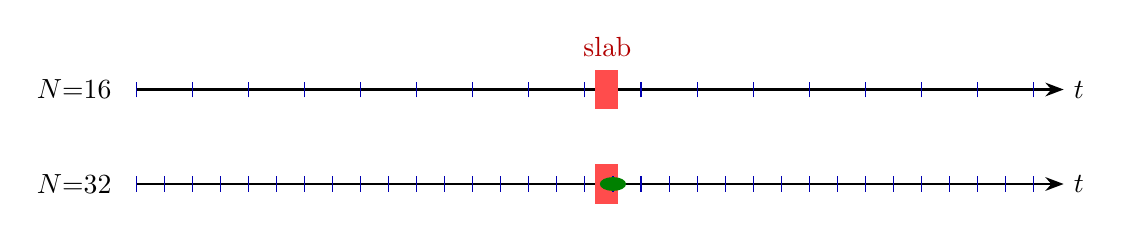
\begin{tikzpicture}[>=Stealth,xscale=1.9]
 \draw[->,thick] (0,0)--(6.2,0) node[right]{$t$};
 \fill[red!70] (3.07,-0.25) rectangle (3.22,0.25);
 \node[red!70!black,above] at (3.15,0.3) {slab};
 % N=16, step 0.375
 \foreach \k in {0,...,16} \draw[blue!70!black] ({\k*0.375},-0.1)--({\k*0.375},0.1);
 \node[left] at (-0.1,0) {$N{=}16$};
 \begin{scope}[yshift=-1.2cm]
  \draw[->,thick] (0,0)--(6.2,0) node[right]{$t$};
  \fill[red!70] (3.07,-0.25) rectangle (3.22,0.25);
  \foreach \k in {0,...,32} \draw[blue!70!black] ({\k*0.1875},-0.1)--({\k*0.1875},0.1);
  \fill[green!50!black] (3.1875,0) circle (2.5pt);
  \node[left] at (-0.1,0) {$N{=}32$};
 \end{scope}
\end{tikzpicture}
\caption{Uniform samples (ticks) vs.\ a slab of width $0.15$. With $N=16$ ($\Delta_t=0.375$) no sample falls inside the slab; with $N=32$ one sample (green) does and the slab is detected.}
\end{figure}

\begin{intuition}
A tilted wall means the ray's path inside the slab depends on the pixel; for some pixels the in-slab path is shorter than the step, and the samples jump over it. That is a classic \emph{aliasing} problem, here producing a regular pattern of missing columns. In a learned volume the thin layer is a surface, so missing it means missing the object.
\end{intuition}

\subsection{Background Radiance\slides{67}}

Reinstate the background wall at $\x_z$:
\[
L(\x,\w)\approx\sum_{i=1}^NT(\x,\x_{t_i})\bigl(1-e^{-\sigma_{t_i}\Delta t_i}\bigr)L_e(\x_{t_i},\w)+T(\x,\x_{t_{N+1}})\,L(\x_z,\w).
\]
The slide's remark: the final transmittance $T(\x,\x_{t_{N+1}})$ can be thought of as a ``\emph{background mask}'' (it is 1 where the ray crossed nothing and 0 where it was fully absorbed).

\begin{intuition}
By Proposition~\ref{prop:unity} the pixel is a convex combination: samples take weight $\sum w_i=1-T_{N+1}$, the background takes $T_{N+1}$. Rendering the mask $T_{N+1}$ alone gives a silhouette image, useful for training with segmentation masks, and for compositing on arbitrary backgrounds.
\end{intuition}

\subsection{Summary\slides{68}}

Slide 68 recaps: the emission--absorption model $\mathrm dL=-\sigma_aL\,\mathrm dz+\sigma_aL_e\,\mathrm dz$; transmittance as $\exp(-\int\sigma)$ (see Fig.\ above); and the computational algorithm $L\approx\sum_iT(\x,\x_{t_i})(1-e^{-\sigma_{t_i}\Delta_t})L_e$ with the recursion for $T$. (Slides 69--71: preview of the next lecture, which is about NeRF-style neural fields, questions and acknowledgements. The slides are adapted from \emph{Learning for 3D Vision}, CMU 16-825, Prof.\ S.~Tulsiani, which credits Yannis Gkioulekas for most slides and figures, Pat Hanrahan for the radiance diagram, Wojciech Jarosz, and Studio Lernert \& Sander.)

%=====================================================================
\section{Summary}
%=====================================================================
\subsection{Comparison of the models covered}

\begin{table}[h]
\centering
\small
\renewcommand{\arraystretch}{1.35}
\begin{tabular}{@{}p{3.1cm}p{4.4cm}p{3.7cm}p{3.5cm}@{}}
\toprule
\textbf{Model} & \textbf{Pixel value} & \textbf{Needs} & \textbf{Limits}\\
\midrule
Surface rendering (slide 14) & $L(\x^*-\lambda\w,\w)$ at the first hit & depth $\lambda$, shading & no fog, smoke, glow\\
Absorption only, homogeneous (42) & $e^{-\sigma z}L(\x_0,\w)$ & constant $\sigma$ & no emission, uniform media\\
Absorption only, heterogeneous (43, 46) & $T(\x,\x_z)L(\x_z,\w)$, $T=e^{-\int\sigma}$ & $\sigma(\x)$ along the ray & no emission\\
Emission--absorption, analytic (51--53) & $e^{-\sigma\Delta}L_{bg}+(1-e^{-\sigma\Delta})C$ & constant $\sigma,C$ & only homogeneous media\\
Emission--absorption, general (49) & $T L_{bg}+\int T\sigma L_e\,\mathrm dt$ & $\sigma(\x),L_e(\x,\w)$ & no closed form; no explicit scattering\\
Ray marching (58--67) & $\sum_iT_i(1-e^{-\sigma_i\Delta t_i})L_{e,i}+T_{N+1}L_{bg}$ & samples along ray & discretisation error, sampling aliasing\\
Full RTE (34) & EA terms plus $-\sigma_sL+\sigma_sL_s$ & $\sigma_s$, phase function $f_p$ & expensive, recursive; allows relighting\\
\bottomrule
\end{tabular}
\caption{Models of increasing generality discussed in the lecture.}
\end{table}

\subsection{A qualitative comparison plot}

Figure~\ref{fig:matrix} summarises which effects each model can capture, following slides 54 and 37: green = natively captured, yellow = only through an arbitrary effective emission $L_e'$ (in principle, with complex inhomogeneous scenes), red = not captured. This is my own qualitative reading of the slides, not a measurement.

\begin{figure}[h]
\centering
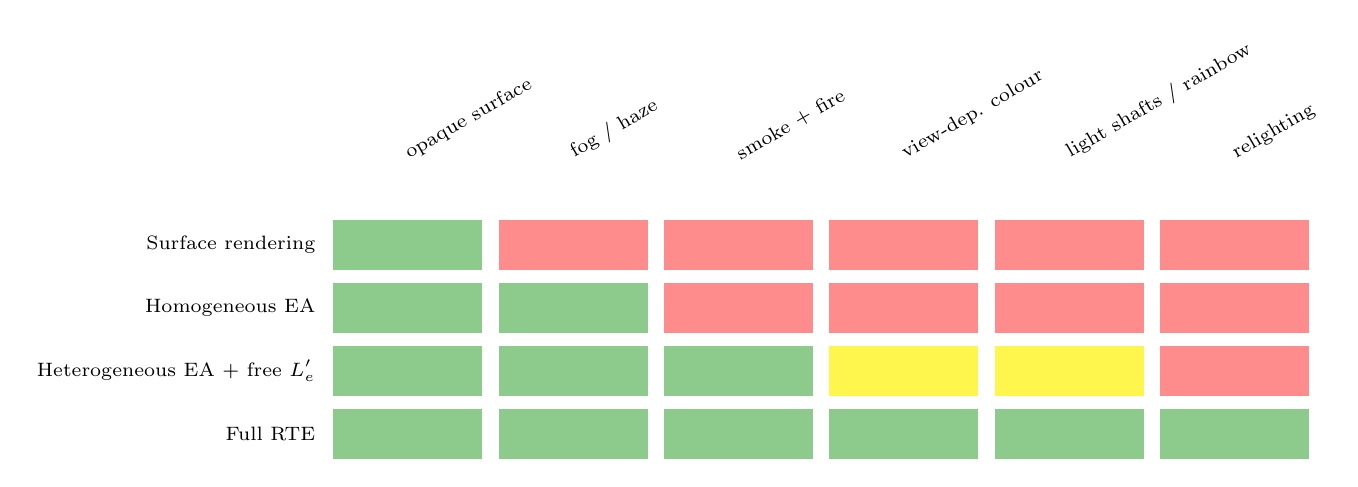
\begin{tikzpicture}[x=2.1cm,y=0.8cm,font=\scriptsize]
 \foreach \e [count=\j from 0] in {opaque surface,fog / haze,smoke + fire,view-dep. colour,light shafts / rainbow,relighting}
   \node[rotate=30,anchor=south west] at (\j,0.1) {\e};
 \foreach \m [count=\i from 1] in {Surface rendering,Homogeneous EA,Heterogeneous EA + free $L_e'$,Full RTE}
   \node[anchor=east] at (-0.5,-\i) {\m};
 \def\cell#1#2#3{\fill[#3] (#2-0.45,-#1-0.4) rectangle (#2+0.45,-#1+0.4);}
 \colorlet{gg}{green!55!black!45}\colorlet{yy}{yellow!70}\colorlet{rr}{red!45}
 \cell{1}{0}{gg}\cell{1}{1}{rr}\cell{1}{2}{rr}\cell{1}{3}{rr}\cell{1}{4}{rr}\cell{1}{5}{rr}
 \cell{2}{0}{gg}\cell{2}{1}{gg}\cell{2}{2}{rr}\cell{2}{3}{rr}\cell{2}{4}{rr}\cell{2}{5}{rr}
 \cell{3}{0}{gg}\cell{3}{1}{gg}\cell{3}{2}{gg}\cell{3}{3}{yy}\cell{3}{4}{yy}\cell{3}{5}{rr}
 \cell{4}{0}{gg}\cell{4}{1}{gg}\cell{4}{2}{gg}\cell{4}{3}{gg}\cell{4}{4}{gg}\cell{4}{5}{gg}
\end{tikzpicture}
\caption{Qualitative capability matrix (green: yes, yellow: in principle via $L_e'$, red: no).}\label{fig:matrix}
\end{figure}

\subsection{Key take-aways}
\begin{itemize}[leftmargin=1.4em]
 \item \textbf{Drop the surface assumption.} Represent the scene by a non-negative density field $\sigma(\x)$ (plus emitted colour); an opaque surface is just the limit of a very sharp density jump.
 \item \textbf{One ODE does most of the work.} The emission--absorption model $\mathrm dL=-\sigma L\,\mathrm dz+\sigma L_e\,\mathrm dz$ integrates to $L=T(\x,\x_z)L_{bg}+\int_0^zT(\x,\x_t)\sigma(\x_t)L_e(\x_t,\w)\mathrm dt$, with transmittance $T=e^{-\int\sigma}$ and its multiplicativity property.
 \item \textbf{Scattering is expensive but can be absorbed in an effective emission} $L_e'=L_e+\tfrac{\sigma_s}{\sigma_a}(L_s-L)$; this is why EA is the de-facto standard in neural volume rendering (at the price of no physical relighting).
 \item \textbf{Ray marching is alpha compositing.} $\alpha_i=1-e^{-\sigma_i\Delta t_i}$, $T_{i+1}=T_i(1-\alpha_i)$, $w_i=T_i\alpha_i$, $L\approx\sum_iw_iL_{e,i}+T_{N+1}L_{bg}$; the weights telescope to $1-T_{N+1}$.
 \item \textbf{Where you sample matters.} Uniform sampling can step over thin dense layers (aliasing); non-uniform sampling spends samples where $\sigma$ is large. Next lecture: combine this renderer with neural representations.
\end{itemize}

\end{document}